% !TeX spellcheck = ru_RU

\chapter{Конструкторская часть}
В этом разделе будут представлено описание используемых типов данных, а также схемы алгоритмов вычисления расстояния Левенштейна и Дамерау-Левенштейна.

\section{Разработка алгоритмов}
В данной части будут рассмотрены схемы алгоритмов нахождения расстояний Левештейна и Дамерау-Левенштейна. На рисунках \ref{fig:leven} --- \ref{fig:damercache} представлены схемы рассматриваемых алгоритмов.
\begin{figure}[h]
	\centering
	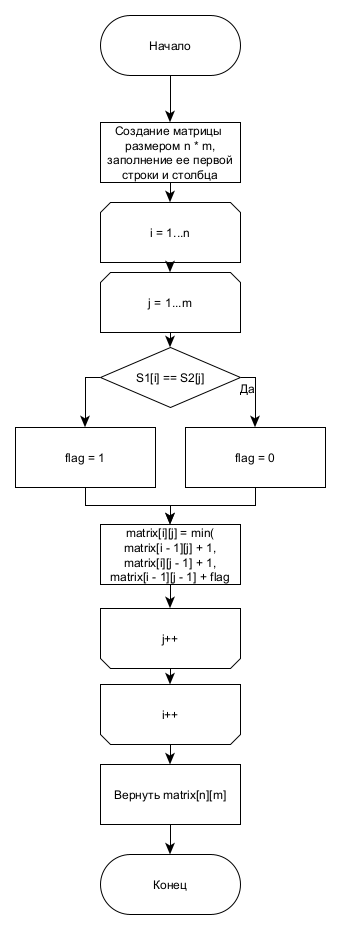
\includegraphics[scale = 0.7]{img/levenshtein.png}
	\caption{Схема алгоритма нахождения расстояния Левенштейна}
	\label{fig:leven}
\end{figure}
\begin{figure}[h]
	\centering
	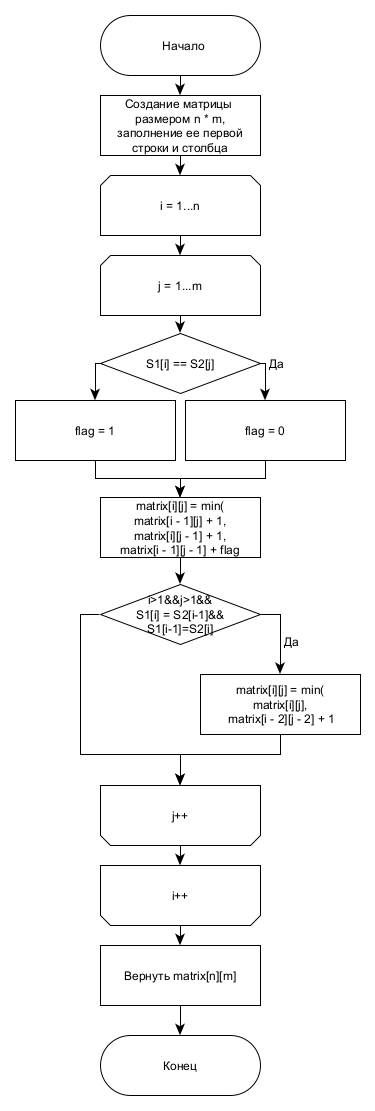
\includegraphics[scale = 0.65]{img/damer.png}
	\caption{Схема матричного алгоритма нахождения расстояния Дамерау-Левенштейна}
	\label{fig:damer}
\end{figure}
\begin{figure}[h]
	\centering
	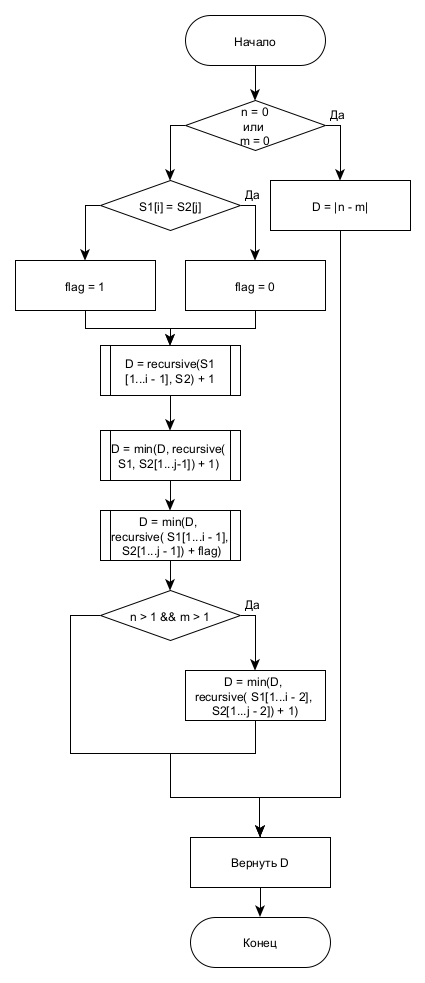
\includegraphics[scale = 0.7]{img/damerrec.png}
	\caption{Схема рекурсивного алгоритма нахождения расстояния Дамерау-Левенштейна}
	\label{fig:damerrec}
\end{figure}
\begin{figure}[h]
	\centering
	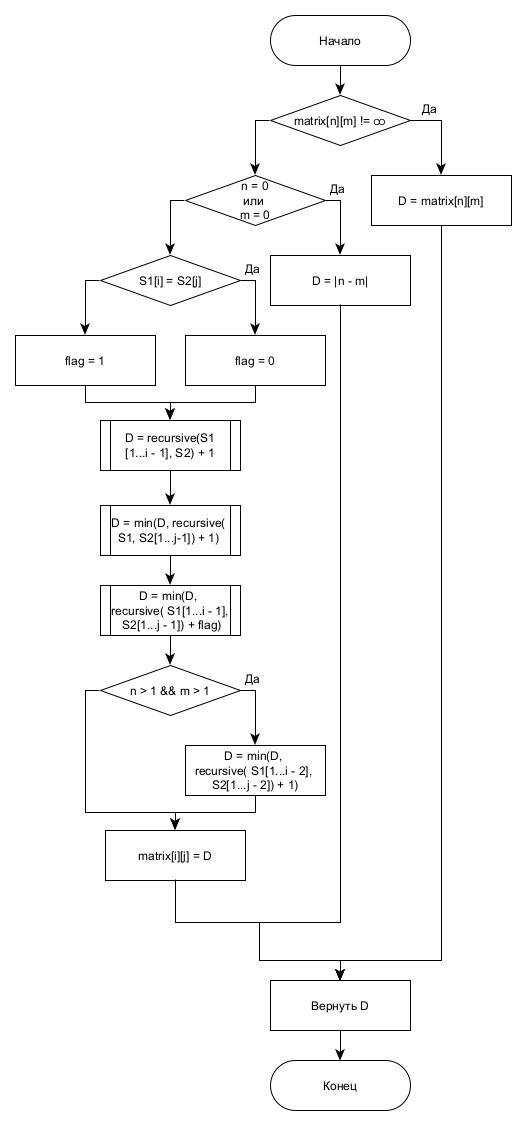
\includegraphics[scale = 0.6]{img/damercache.png}
	\caption{Схема рекурсивного алгоритма нахождения расстояния Дамерау-Левенштейна с использованием кэша}
	\label{fig:damercache}
\end{figure}
\clearpage


\section*{Вывод}
На основе теоретических данных, полученных в аналитическом разделе, были построены схемы исследуемых алгоритмов.